%!TEX root=../document.tex
\section{Loadbalancing - Allgemein}
Lastverteilung wird verwendet, wenn mit einer Vielzahl von Anfragen gerechnet wird, und diese entsprechend auf verschiedene Server verteilt werden sollen.

Loadbalancing beschreibt also wie die Last in Form von Clientzugriffen auf verschiedene Server aufgeteilt wird.
Lastverteilung wird in fast jedem größerem System implementiert, wobei zu unterscheiden ist, welche Methode der Lastverteilung angewendet wird. (Round Robin, Weighted Round Robin usw.)

Ein Loadbalancing System ist meist wie folgt aufgebaut:

\begin{figure}[!h]
\centering
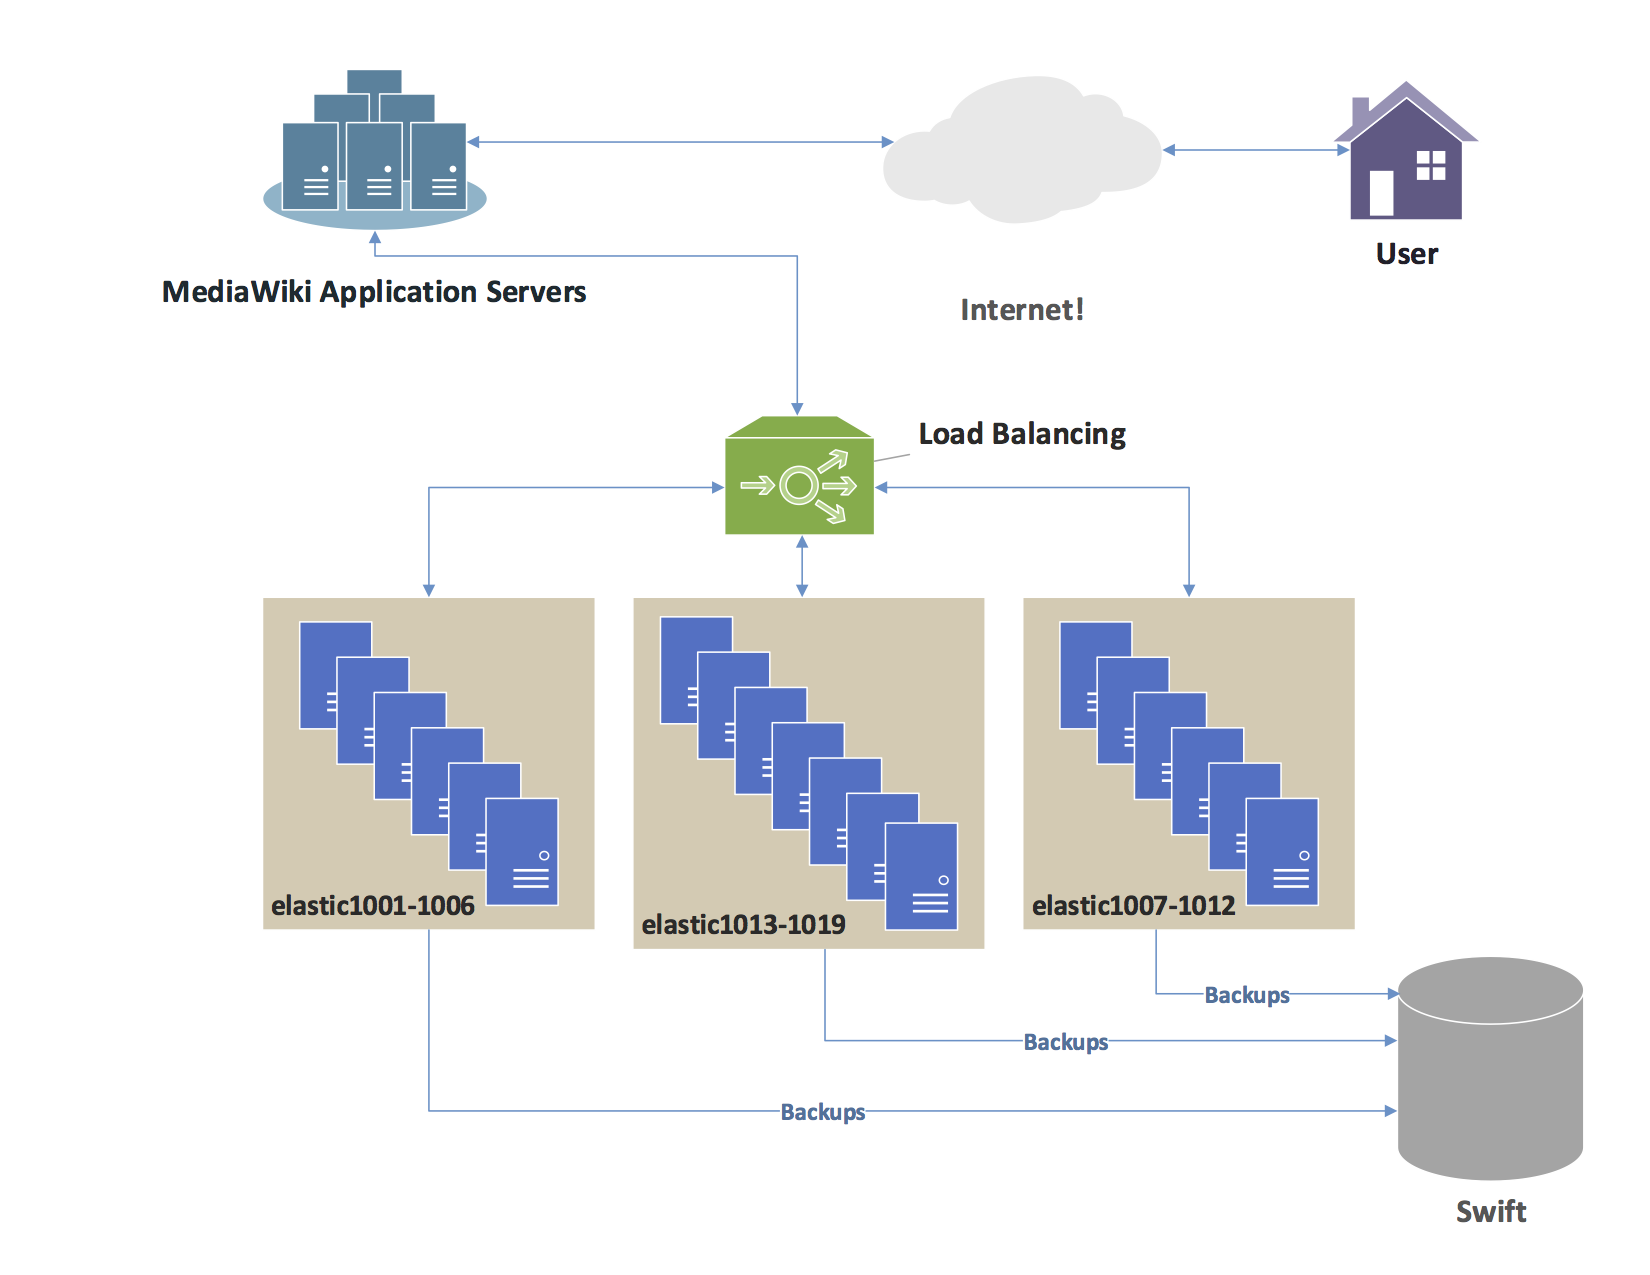
\includegraphics[width=0.7\linewidth]{images/load}
\caption[Loadbalancing schema]{Loadbalancing schema \cite{wiki}}
\label{fig:load}
\end{figure}

In diesem Beispiel versucht ein Client auf den Inhalt der MediaWiki Server zuzugreifen. Anstatt diesen Client direkten Zugang zu der Kommunikation mit einem ausgewähltem Server zu geben, wird zwischen der Verbindung zwischen Client und Server ein Loadbalancer geschalten.

Dieser ist dafür zuständig jegliche Kommunikation entgegen zunehmen und entsprechend nach der eingestellten balance Methode die last auf den passenden Server aufzuteilen.

Bei diesem Vorgang darf selbstverständlich die Session zwischen User und Server nicht ''verloren'' gehen. Um die Session Persistence zu garantieren muss der Loadbalancer einen verbundenen Client mit dem entsprechenden Server in Verbindung bringen.

\section{Ergebnisse}
Für die Kommunikation zwischen Server und Client wurde RMI (Remote Method Invocation) gewählt. Um das Testen sowie die Simulation von Clients und Server zu vereinfachen, wurde das Starten der Clients und entsprechenden Server simuliert.

Ein Balancing mit konkreten Server VMs wäre mit dem erstellten Code prinzipiell möglich. Es müsste lediglich ein Pool von Adressen ausgewählt werden und den jeweiligen Servern zugeteilt werden.

\subsection{Kommunikation mittels RMI}
RMI (Remote Method Invocation) beschreibt den Aufruf einer Methode eines entfernten Java – Objektes. Dabei kann sich das Objekt in einer vollkommen anderen JVM befinden.

Meistens wird RMI als Client / Server Prinzip umgesetzt, das heisst wir haben einen Client, welcher eine bestimmte (meist komplexe) Tätigkeit, erledigen will. Dafür stellen wir ihm einen Server bereit, welcher die Ressourcen und die Mittel dazu hat diese Tätigkeit zu übernehmen.
Ein typisches server Programm erstellt mehrere remote Objects, referenziert auf diese bzw. übermittelt sein Skeleton, und wartet bis diese Clients seine Methoden aufrufen.

Ein typisches client Programm erhält eine reference eines remote Servers zu einem oder mehreren remote Objekten und ruft anschließend mittels Sockets über das Skeleton des Servers die gewünschten Methoden auf.

RMI bietet (in Java) den Grundmechanismus bei dem der Server und der Client, untereinander Informationen austauschen können (meist unter Verwendung von Sockets). So eine Art von Programm wird oft als distributed Object application bezeichnet.

\subsubsection{Aufbau von RMI}

\begin{figure}[!h]
\centering
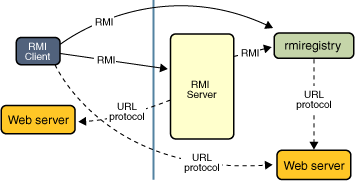
\includegraphics[width=0.46\linewidth]{images/rmi}
\caption{RMI Aufbau}
\label{fig:rmi}
\end{figure}

Folgende Abbildung beschreibt eine Applikation welche den Mechanismus von RMI implementiert.

Es wird eine RMI Registry verwendet um die Refernzen eines Remote Objects zu erlangen. Der Server ruft die Registry auf bzw binded sie. Somit wird gleichzeitig ein Name für das Remote Object gebindet.

Der Client sucht nach dem gebindeten Remote Object in der Registry des Servers und invoked anschließend die gewünschte Methode/Methoden davon.
Ebenfalls wird gezeigt, dass das RMI system einen existierenden Web Server benützt um Klassen Definitionen zu laden. Von dem Server auf den Client und von dem Client auf dem Server wenn gebraucht. 

\subsubsection{Klassenaufteilung / Architektur}
Um die Anforderungen zu erfüllen wurde folgende Klassenstruktur umgesetzt. Zur Darstellung der Architektur wurde ein entsprechendes UML - Diagramm beigelegt.
\begin{figure}[!h]
	\centering
	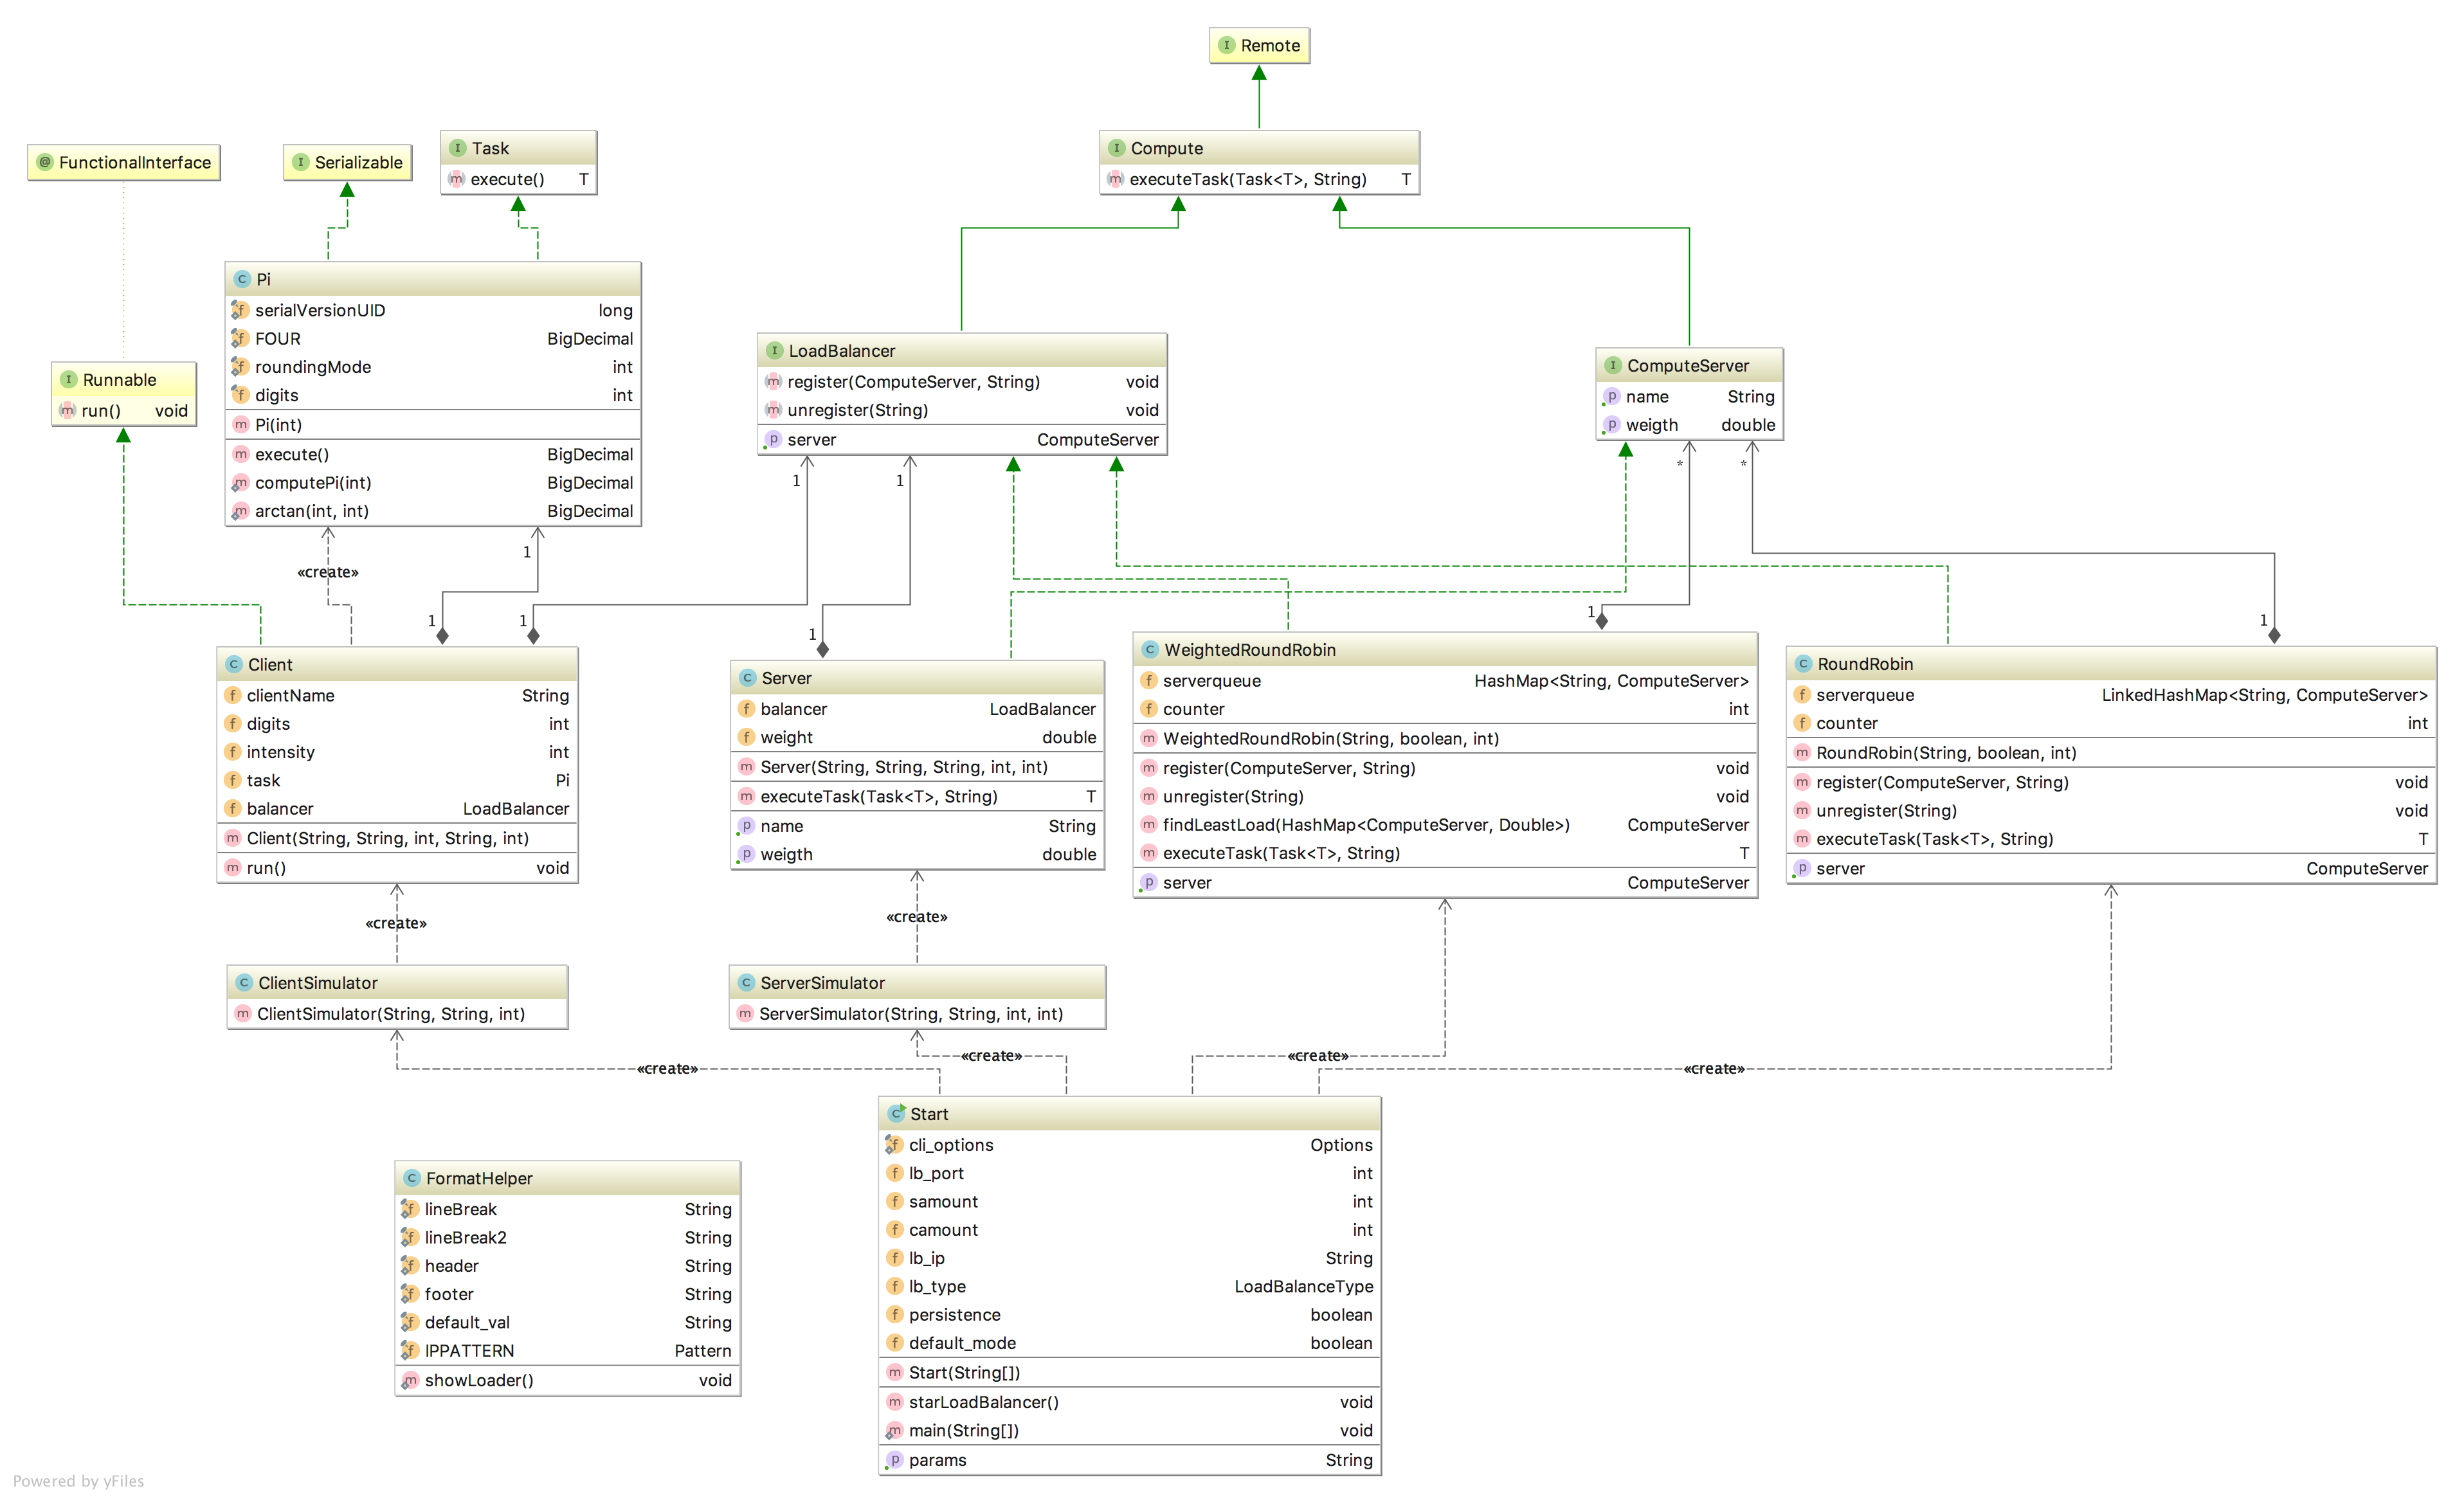
\includegraphics[width=1\linewidth]{images/diagram}
	\caption{}
	\label{fig:diagram}
	
\end{figure}

\subsection{CLI Parsing - Usage}
Damit alle benötigten Parameter ohne Mehraufwand angegeben werden können, haben wir uns für den ''\textit{commons cli Parser}'' von Apache.org entschiedene.

Parameter wie Loadbalancer Ip oder Anzahl der Clients/Server können somit entsprechend eingestellt werden.

Die Usage sieht wie folgt aus:
\begin{lstlisting}[style=Java, caption=Usage]	
java Start [-d] -s 10 -c 10 -t RR -l 127.0.0.1 -p
\end{lstlisting}

\begin{itemize}
	\item \textbf{Client Amount -c}\\
	Angabe eines int wertes entspricht der Anzahl der generierten Clients.
	
	\item \textbf{Server Amount -s}\\
	Angabe eines int wertes entspricht der Anzahl der generierten Server.
	
	\item \textbf{Balance Type -t}\\
	Wählen des entsprechendes Loadbalancers
	\begin{itemize}
		\item \textbf{RR} - Round Robin
		\item \textbf{WR} - Weighted Round Robin
	\end{itemize}
	
	\item \textbf{Balancer IP -l}\\
	IP-Addresse des Loadbalancers bzw. der RMI Registry
	
	\item \textbf{Persistence -p}\\
	Wenn angegeben, dann wird die Session persisitert
	
	\item \textbf{Default -d}\\
	Wenn angegeben werden alle nicht angegebenen Werte mit dem Default Wert belegt.
\end{itemize}

\clearpage

\subsubsection{Compute Package}
Das Compute Package ermöglicht das erstellen von generischen Tasks.
Dazu gibt es das Compute und das Task Interface. 
Das Task Interface definiert einen generischen Task mit einer Methode, die einen generischen Wert zurückgibt. 

\begin{lstlisting}[style=Java, caption=generic Task Interface]	
public interface Task<T> {
	T execute();
}
\end{lstlisting}

Möchte ein Server einen generischen Task ausführen können muss er das Compute Interface implementieren. 

\begin{lstlisting}[style=Java, caption=Compute Interface]	
public interface Compute extends Remote {
<T> T executeTask(Task<T> t, String clientName) throws RemoteException;
}
\end{lstlisting}

Mithilfe von diesem kann der Task über RMI ausgeführt werden. 

\clearpage
\subsubsection{Loadbalancer generell}
Grundsätzlich hat ein LoadBalancer durch das Interface folgende Methoden vorgegeben: 
\begin{lstlisting}[style=Java, caption=Loadbalancer Interface]	

public void register(ComputeServer c, String name)  throws RemoteException;

public void unregister(String name) throws RemoteException;

public ComputeServer getServer() throws RemoteException;

\end{lstlisting}

Somit kann der LoadBalancer neue Server registrieren sie wieder entfernen und einen Server für den Client aussuchen. 
Die getServer hat also je nach LoadBalancer-Art einen neuen Algorithmus.

\subsubsection{Loadbalancer Round Robin}
RoundRobin benutzt einen sehr einfachen Algorithmus. Dabei wird einfach aus einer Liste der Reihe nach immer ein anderer Server ausgewählt. 
\begin{lstlisting}[style=Java, caption=RoundRobin Konstruktor]	
 public RoundRobin(String name, boolean persistance, int port){
	this.serverqueue=new LinkedHashMap<String,ComputeServer>();
	int counter=0;
	
	//registering Object to RMI
	try{
		LoadBalancer stub = (LoadBalancer) UnicastRemoteObject.exportObject(this, port);
		
		Registry r = LocateRegistry.createRegistry(port);
		r.bind(name,stub);
	} catch (RemoteException e) {
		System.err.println("RemoteException Ocurred");
	} catch (AlreadyBoundException e) {
		System.err.println("Some Object is allready bound at the name: "+name);
	}
	
}
\end{lstlisting}

Um die Server zu speichern wurde eine LinkedHashMap benutzt. Diese hält die Werte in eingefügter Reihenfolge. Somit kann Servername mit den Server Objekt gematcht werden und auch sehr einfach über die Liste iteriert werden. 
Weiters wird das Objekt an die Registry gebunden um RMI zu ermöglichen. 

register und remove fügen einfach Elemente in die LinkedHashMap hinzu oder entfernen sie wieder. 

\begin{lstlisting}[style=Java, caption=RoundRobin getServer]	
  public ComputeServer getServer() throws RemoteException {
	Iterator<ComputeServer> servers=this.serverqueue.values().iterator();
	for(int i=0;i<counter;i++){
		if(servers.hasNext()) {
			servers.next();
		}
	}
	counter=(counter+1)%this.serverqueue.size();
	
	return servers.next();
}
\end{lstlisting}

Der LoadBalancer hat einen Counter. Jedes Mal wenn ein neuer Aufruf auf einen Server erfolgt wird dieser um 1 erhöht. 
Der Wert des Counters bewegt sich immer zwischen 0 und der Mapgröße-1.
Mithilfe eines Iterators und einer for-Schleife wird dann immer der nächste Server ausgewählt. 

\begin{lstlisting}[style=Java, caption=RoundRobin getServer]	
public ComputeServer getServer() throws RemoteException {
Iterator<ComputeServer> servers=this.serverqueue.values().iterator();
for(int i=0;i<counter;i++){
if(servers.hasNext()) {
servers.next();
}
}
counter=(counter+1)%this.serverqueue.size();

return servers.next();
}
\end{lstlisting}
Der generische Task des Clients wird einfach an den jeweiligen Server weitergeleitet. 


\subsubsection{Loadbalancer Weighted Round Robin}
Weighted Round Robin basiert auf dem Prinzip von Round Robin.
Es werden ebenfalls die Server gewechselt, jedoch wird eine Gewichtung mit einbezogen, welche entweder statisch für jeden Server vergeben wird, oder durch die aktuelle Auslastung (RAM, CPU generell System Load) berechnet.

In unserem Fall wurde die RAM Last mit in die Berechnung einbezogen.

Ähnlich wie bei Round Robin wird eine Map generiert, welche die gegebenen Server sowie deren Name in einer Map speichert.
Vor jedem Berechnungsvorgang wird die Serverlast jedes einzelnen Servers berechnet und anschließend in einer entsprechenden Liste mit der aktuellen Serverlast als long wert gespeichert.
Nach der Berechnung wird die geringste Serverlast entnommen und als verfügbarer Server angeboten.

\begin{lstlisting}[style=Java, caption=Weighted Round Robin Lastberechnnug]	
@Override
public ComputeServer getServer() throws RemoteException {
	HashMap<ComputeServer, Double> weightedMap = new HashMap<>();
	
	Iterator<String> it = this.serverqueue.keySet().iterator();
	while (it.hasNext()) {
		ComputeServer server = this.serverqueue.get(it.next());
		double weightTemp = server.getWeigth();
		weightedMap.put(server, weightTemp);
	}
	
	return this.findLeastLoad(weightedMap);
}

private ComputeServer findLeastLoad(HashMap<ComputeServer, Double> weightedMap) {
	Map.Entry<ComputeServer, Double> min = null;
	for (Map.Entry<ComputeServer, Double> entry : weightedMap.entrySet()) {
		if (min == null || min.getValue() > entry.getValue()) {
			min = entry;
		}
	}
	return min.getKey();
}
\end{lstlisting}

Nachdem ein entsprechender Server gefunden wurde wird dieser an den anfragenden Client mittels RMI (Remote Method Invokation) übergeben.

Anschließend werden durch die implementierte Session Persistence alle offenen Server - Client verbindungen aufrecht erhalten.

\clearpage

\subsubsection{Serverseite}
Auf der Serverseite gibt es grundsätzlich das Interface Compute Server. Dieses definiert die 2 Methoden die wichtig für einen Server ist, der Tasks berechnen soll. 
getName() und getWeight()

Die Klasse Server implementiert dann einen funktionsfähigen Server. 

\begin{lstlisting}[style=Java, caption=Server Implementierung]	
public Server(String loadbalancerIp, String loadbalancerName, String servername, int port, int weight) {
	this.name = servername;

	try {
	Registry registry = LocateRegistry.getRegistry(loadbalancerIp, port);
	this.balancer = (LoadBalancer) registry.lookup(loadbalancerName);
	} catch (RemoteException e) {
		System.err.print("Remote Exception occured");
	} catch (NotBoundException e) {
		System.err.println("There was no bound loadbalancer under this name");
		System.exit(-1);
	}
	try {
		ComputeServer stub = (ComputeServer) UnicastRemoteObject.exportObject(this, port);
		this.balancer.register(stub, this.name);
	} catch (RemoteException e) {
		e.printStackTrace();
	}

}
\end{lstlisting}

Der Server kann sich die Registry, welche für RMI nötig von der IP holen bei der auch der Loadbalancer liegt.
Danach kann er sich mithilfe des Namen des Loadbalancers das Objekt von der Registry holen. 
Nachdem das erfolgreich war muss der Server sich selbst für den Remote Zugriff verfügbar machen. 
Dazu muss ein stub erstellt werden. Dieser wird dann dem LoadBalancer übergeben. 
Somit kann der LoadBalancer dann auf den Server zugreifen. 

Weiters kann der Server mit getWeight sein Gewicht berechnen. Dies erfolgt mithilfe der RAM Auslastung und einem zufälligen Wert für Simulationszwecke. 

\clearpage

\begin{lstlisting}[style=Java, caption=Server getWeight]	
  public double getWeigth() throws RemoteException {
	int ram = 0;
	Runtime runtime = Runtime.getRuntime();
	long ram_availiabe = runtime.totalMemory();
	long ram_used = runtime.totalMemory() - runtime.freeMemory();
	ram = (int) (((100.0 / (double) ram_availiabe) * (double) ram_used) + 0.5);
	
	double sysload = Double.NaN;
	OperatingSystemMXBean mx;
	try {
		mx = ManagementFactory.getOperatingSystemMXBean();
		sysload = mx.getSystemLoadAverage();
	} catch (Throwable t) {
		t.printStackTrace();
	}
	
	double weight = (int)(Math.random()*100)+1;
	weight = weight + (ram/2);
	weight+=sysload;
	this.weight = weight;
	System.out.println(this.name + "has the weight " + weight);
	return weight;
}
\end{lstlisting}


Die Klasse ServerSimulator ist nur dazu da um eine gewünschte Anzahl an Servern zu erstellen:


\begin{lstlisting}[style=Java, caption=Server Simulator]	
public class ServerSimulator {
	public ServerSimulator(String lb_ip, String loadbalancer, int samount, int lb_port) {
		for (int i=0; i<samount; i++) {
			//new Server(lb_ip, loadbalancer, samount, "Server"+(i+123322));
		new Server(lb_ip, loadbalancer,  "Server"+(i), lb_port, i);
		}
	}
}

\end{lstlisting}

\clearpage

\subsection{Clientseite}
Nachdem die Clients mithilfe des Clientsimulator gestartet wurden, wird automatisch eine Intensity von 4-Anzahl der Clients vergeben.

Anschließend wird je nach Intensity eine Anfrage an den entsprechenden LoadBalancer gestellt, welcher anschließend den jeweiligen Server auswählt und den gewünschten Task ausführt.

Somit hat der Client nur Zugriff auf den Loadbalancer, übermittelt den gewünschten Task und erhält anschließend das Ergebnis.

\begin{lstlisting}[style=Java, caption=Clientseite RMI Connection]	
// Fetchen des Loadbalancers aus der Registry
try {
	Registry registry = LocateRegistry.getRegistry(loadbalancerIp);
	this.balancer = (LoadBalancer) registry.lookup(loadbalancerName);
	this.task = new Pi(digits);
} catch (Exception e) {
	System.err.println("ComputePi exception:");
	e.printStackTrace();
}

// Starten des Client Threads
Thread client_thread = new Thread(this);
client_thread.start();
\end{lstlisting}

Nachdem der ClientThread gestartet wurde, wird mit der entsprechenden Intensity (simuliert durch ein Thread.sleep()) endlos eine Anfrage an den LoadBalancer geschickt.

Die Anfrage ist in diesem Beispiel die Berechnung von Pi mit einer zufälligen Anzahl von Nachkommastellen.

\begin{lstlisting}[style=Java, caption=Client Thread]	
public void run() {
	while (true) {
		try {
			Thread.sleep(this.intensity*1000);
		
			BigDecimal pi = this.balancer.executeTask(this.task, this.clientName);
			
			} catch (InterruptedException e) {
				e.printStackTrace();
			} catch (RemoteException e) {
				e.printStackTrace();
		}
	}
}
\end{lstlisting}
